\chapter{\label{a:control}Control considerations}
Control is an essential aspect of gravitational wave interferometry, with the noise sources described in Section\,\ref{sec:ifo-noise} combining to push the test masses away from the operating point.

\section{\label{sec:snr}Signal to noise ratio}
Signal cannot be measured below the noise present on a photodetector. Maximum sensitivity can be achieved by maximising the ratio of signal power, $S$, to noise power, $N$, in the frequency band of interest. This is expressed as the \emph{signal-to-noise} ratio (SNR),
\begin{equation}
  \text{SNR} = \frac{S}{N}.
\end{equation}
When discussing controls, the standard representation of signal to noise is in units of \emph{decibels} (\SI{}{\deci\bel}), defined for signal power as:
\begin{equation}
  \text{SNR}_{\SI{}{\deci\bel}} = 10 \log_{10} \left( \frac{S}{N} \right).
\end{equation}
As this representation is logarithmic, it is a useful for expressing both small and large signals and is therefore suitable for the presentation of noise sources across many orders of magnitude, as with interferometry.

\note{Define SNR for signal amplitude?}

\section{\label{sec:freq-resp-signals}Frequency representation of signals and noise}
\subsection{\label{sec:fourier-transform}Fourier transform}
A Fourier transform represents a time-varying signal in terms of its frequency components, i.e. as a series of sinusoidal waves of different frequency and amplitude. The Fourier transform $x \left( f \right)$ of $x \left( t \right)$ can be defined as:
\begin{equation}
  \label{eq:fourier-transform}
  x \left( f \right) = \int^{\infty}_{-\infty} x \left( t \right) \text{e}^{-2i \pi f t} dt.
\end{equation}
Noise transients that appear in a detector have finite energy over a finite time, and can be entirely characterised by a Fourier transform of the time series in which the event occurred. Other forms of noise, however, cannot be represented in this way.

\subsection{Spectral density}
Apart from noise transients, the remaining noise sources within the interferometer tend to arise from stationary, random processes. This means that the noise source's \emph{autocorrelation}\textemdash its self-similarity over time\textemdash is zero for all times greater than zero. The energy of this noise approaches infinity as measurement time approaches infinity. In this circumstance, the Fourier transform of the underlying time-domain signal, as shown in Section\,\ref{sec:fourier-transform}, does not strictly exist. An alternative representation of a noise process is to represent the amount of work it performs per unit time: its power. The \emph{power spectral density} is a representation of the power present within each frequency of a signal in the steady state.

The infinite time Fourier transform in Equation\,\ref{eq:fourier-transform} can be truncated to instead represent the frequency components within a certain window:
\begin{equation}
  x \left( f \right) \approx \frac{1}{\sqrt{T}} \int^{T}_{0} x \left( t \right) \text{e}^{-2i \pi f t} dt,
\end{equation}
and the power spectrum of the signal measured by a photodetector is then:
\begin{equation}
  \label{eq:psd}
  S_{xx} = \frac{1}{T} \int^{T}_{0} x \left( f \right)^2 dt.
\end{equation}
Remembering that photodetectors measure power (Section\,\ref{sec:operating-point}), this means that the photodetector's power spectrum would have units of \SI{}{\watt^2\per\hertz}. At the operating point, the photodetector's power is arranged in such a way as to be a linear with cavity mirror displacement, and so a more useful unit is the \emph{amplitude spectral density} $A \left( f \right)$, which is simply the square root:
\begin{equation}
  A \left( f \right) = \sqrt{S_{xx} \left( f \right)},
\end{equation}
which for the photodetector would have units \SI{}{\watt\per\sqrthz}.

\subsection{\label{sec:windowing}Estimation of spectral density}
Equation\,\ref{eq:psd} gives the formal definition of the power spectral density but not a practical means to measure it. To estimate the frequency components of a measured photodetector signal, we employ \emph{spectral density estimation} techniques. The standard in experimental interferometry is Welch's method \cite{Welch1967}, which splits a measured time series into a series of segments which can overlap with adjacent segments before calculating Fourier transforms on each individual segment. The resulting Fourier transforms are recombined to produce the spectral density estimate.

The segment period determines the lowest frequency resolved by the calculation. For instance, a segment length of \SI{1000}{\second} would result in frequency resolution down to $\frac{1}{1000} = \SI{e-3}{\hertz}$. Segmentation can be used to trade bandwidth for resolution. Instead of taking a segment equal to the signal's period, and therefore achieving resolution at the lowest possible frequencies, segments of shorter duration can be combined to produce better resolution but only at higher frequencies.

Once a segment is created, the resulting Fourier transform is applied to the time series with the assumption that the end cycles back to the start. If the data is noisy, or if the period is not an integer number of wavelengths of all of frequency components, then this creates discontinuities which lead to unphysical frequency domain content (\emph{spectral leakage}). A \emph{window function} can be applied to emphasise the signal in the middle of the segment at the expense of that of the edges. The window function typically used in the field is the Hanning window. The effect of windowing is shown in Figure\,\ref{fig:fft-windowing}. A sine wave of frequency \SI{2499}{\hertz} and unity amplitude is recorded for a period of \SI{1}{\second}, sampled at a frequency of \SI{10}{\kilo\hertz}. The signal frequency is intentionally chosen to avoid an integer multiple of the sample frequency, which would remove the discontinuities at the edge of each segment. The power spectral density has been estimated using Welch's method, with both Hanning windows and flat (\emph{boxcar}) windows. The estimate for the noise floor in each case is drastically different because of the effect of segment discontinuities.
% good windowing description: http://www.ni.com/white-paper/4844/en/

\begin{figure}
  \centering
  \includegraphics[width=\columnwidth]{graphics/generated/from-python/AB-fft-windowing.pdf}
  \caption[The effect of windowing on a power spectral density estimate]{\label{fig:fft-windowing}The effect of windowing on a power spectral density estimate. The underlying signal time series is a sine wave of frequency \SI{2499}{\hertz}, and the sample rate is \SI{10}{\kilo\hertz}. The power spectral density estimates have been made using both Hanning windows, which de-emphasise the start and end of each segment to suppress discontinuities, and a flat window which performs no relative scaling of the data points. Both methods recover the signal's frequency, but in the former case the noise floor is greatly reduced.}
\end{figure}

\section{\label{sec:rms-amplitude}Root mean square amplitude}
A real actuator or sensor has finite range, and the sum of the signal spectral density must be within this range to avoid clipping. The signal in the time domain represents the \emph{root-mean-square} (\gls{RMS}) value of the signal, which is equal to the sum of the frequency components. The \gls{RMS} representation is a useful form for the calculation of required actuator and sensor dynamic range (see, for example, Chapter\,\ref{c:speedmeter-control}).

The following equation converts a power spectral density defined up to $f_{\text{max}}$ to an equivalent \gls{RMS} value:
\begin{equation}
  \label{eq:spectral-density-to-rms}
  x_{\text{rms}}^2 = \int^{f_{\text{max}}}_{0} S_{xx} \left( f \right) df.
\end{equation}
The \gls{RMS} representation of a spectral density is sometimes quoted with the lower integral limit in Equation\,\ref{eq:spectral-density-to-rms} set to \SI{1}{\hertz}, and as such this value represents the signal ``in a \SI{1}{\hertz} band''.

It is advisable to avoid pushing the \gls{RMS} signal applied to a sensor or actuator too close to its limit. Stationary random noise follows a well defined mean but can contain infrequent, larger noise transients allowed by Gaussian statistics. In such a case the instantaneous signal on a sensor or actuator might be greater than the \gls{RMS}. A good rule of thumb is to keep the \gls{RMS} signal expected at a sensor or actuator a factor of about \num{10} below its range to account for such events.

\section{\label{sec:control-loops}Control loops}
A control loop can be used to sense the error in an interferometer from its operating point, and feed back signals to the actuators to correct it. We can in general split a control loop into two distinct parts: the \emph{plant} $G$, which is the device under control, and the \emph{controller} $H$, which is the device that senses the plant's error and generates the corrective feedback. Noise entering the loop between the plant and the controller's input (the \emph{error point}) is termed \emph{sensing} noise, and noise entering between the controller's output and the plant (the \emph{feedback point}) is called \emph{feedback} noise, or, in terms of interferometer test masses, \emph{displacement} noise. Figure\,\ref{fig:control-loop} shows this scenario.

\begin{figure}
  \centering
  \includegraphics[width=\columnwidth]{graphics/generated/from-svg/AB-control-loop.pdf}
  \caption[A basic control loop]{\label{fig:control-loop}A basic control loop. The plant contains the dynamics of the device to be controlled, such as an interferometer. The set position determines the desired point at which the plant should be held, and the error point shows the real position of the plant. The controller generates a corrective signal from the error signal input, and this is the feedback point. Noise enters the system at both the sensing and feedback points.}
\end{figure}

The controller cannot measure errors below its sensing noise and so sensing noise is not suppressed by the control loop.

\subsection{Control loop figures of merit}
A functioning control loop will suppress feedback noise by a level determined by the \emph{open-loop gain}, defined as the product of $G$ and $H$. This can be calculated by breaking the loop and taking a transfer function between the broken edges, and it shows the combined effect the the system under control, its actuators and sensors have on their inputs at their outputs.

The \emph{closed-loop gain} is the effect that the control loop has on the system when negative feedback is being applied. If the controller is able to sense errors and fully correct them, then the closed-loop gain is unity. The frequency domain representation of the closed-loop gain is useful to visualise at which frequencies the gain from the controller is not being applied: closed-loop gain higher than \num{1} shows that the system is not controlling the error point  by matching it with equal magnitude and opposite sign, but rather following it. The closed-loop gain becomes particularly useful when comparing the effect of gain hierarchy, where multiple actuators are used to correct a single error point, as shown in Section\,\ref{sec:sus-gain-hierarchy}.

The neither the open- nor closed-loop gain figures show the explicit effect the controller has on the plant, which in the case of an interferometer would be the positions of the test masses. The \emph{out-of-loop gain} provides this information, and is equal to the error point of the plant when the control loop is enabled. This figure is what is typically plotted in noise budgets such as the one shown in Figure\,\ref{fig:aligo-noise-budget}.

\subsection{\label{sec:control-bandwidth}Control bandwidth}
As discussed in Section\,\ref{sec:rms-amplitude}, actuators and sensors have finite range. When designing a control system for an interferometer, or indeed any plant, the decision must be made between magnitude of the corrective feedback at some frequencies of interest, and the bandwidth over which the plant is to be controlled. For example, a ground-based interferometer typically oscillates with greatest amplitude at frequencies below \SI{1}{\hertz} due to seismic noise, as discussed in Section\,\ref{sec:seismic-noise}. Meanwhile, the shot noise at higher frequencies is small enough such that the test masses do not move away from the operating point. Ideally, the finite actuator range on the test masses should be used to correct for displacements at low frequencies, where it is needed to keep the interferometer at the operating point. To achieve this, the control loop must limit the bandwidth to prevent feedback at high frequencies and enhance feedback at low frequencies. Figure\,\ref{fig:bandwidth} shows the effect that two control servos have given the same ability (e.g. actuator range). By shaping the controller to increase the low frequency gain, the maximum frequency at which feedback is provided (the unity gain frequency \note{make sure this is defined somewhere}) is necessarily reduced. The only way to enhance feedback effort whilst retaining bandwidth is to enhance the range of the actuators and/or sensors.

\begin{figure}
  \centering
  \includegraphics[width=\columnwidth]{graphics/generated/from-python/AB-bandwidth.pdf}
  \caption[Limiting a servo to enhance gain in a certain band]{\label{fig:bandwidth}Limiting a servo to enhance gain in a certain band. The figure shows the loop gain of two servos, each consisting of a simple low pass filter. The area under each transfer function is equal, and this represents the ability of the controller to make corrections to the system (for example, the range of an actuator). To enhance the gain by a factor of \num{10} at \gls{DC}, the unity gain frequency has to be reduced by the same factor, meaning that the system will be controlled over a smaller bandwidth but with greater effort.}
\end{figure}

\subsection{\label{sec:gain-phase-margin}Stable loops}
The stability of a control loop is determined by the controller's ability to generate a corrective signal that is opposite in sign to the disturbance. The interaction between the controller and the plant and its actuators and sensors can in some circumstances create situations where the feedback signal has the same sign as the error signal. If the feedback is of similar magnitude to the error signal, or greater, then this situation leads to positive feedback which makes the system uncontrollable, or \emph{unstable}. In terms of magnitude and phase, this means that any points of unity gain in the transfer function's magnitude must not be coupled with a corresponding phase of \SI{-180}{\degree}. To allow for some uncertainty in the system dynamics, a good rule of thumb in the implementation of the control system is to allow for a \emph{phase margin} of around \SI{35}{\degree} \cite{Freise2003}, meaning that the phase at each unity gain point should not be lower than \SI{-155}{\degree}.